\chapter{Η Υλοποίηση}
\label{ch:Implementation}

\newcommand{\myTTT}[1]{\texttt{\hyphenchar \font=`\- \spaceskip=.5em plus .5em \xspaceskip=.5em #1}}

Υλοποιήσαμε όλους τους αλγορίθμους που αναφέραμε στο Κεφάλαιο \ref{ch:Algorithms} και σχεδιάσαμε μια γραφική διαπροσωπεία για την οπτικοποίηση της εισόδου και των
αποτελεσμάτων. Η υλοποίηση έγινε στη γλώσσα προγραμματισμού \textbf{Python 3} και η οπτικοποίηση με την βιβλιοθήκη \textbf{PyVis}\cite{pyvis-docs}

\section{Οργάνωση Κώδικα}

Η γενική αρχιτεκτονική για την επίλυση του κάθε αλγορίθμου είναι η ίδια σε κάθε περίπτωση. Πιο συγκεκριμένα η υλοποίηση οργανώνεται στα αρχεία: 
\begin{itemize}
	\item \myTTT{main.py} : η αρχή του εκτελέσιμου προγράμματος.
	
	\item \myTTT{graph.py} : η διευθύνουσα κλάση του γραφήματος.
	
	\item \myTTT{polynomial\_time\_algorithm.py} : η διευθύνουσα κλάση για την υλοποίηση του αλγορίθμου.
	 
\end{itemize} 

Επιπλέον αρχεία υλοποιούν κλάσεις οι οποίες είναι απαραίτητες για την υλοποίηση των επιμέρους αλγορίθμων. Αναλυτικά θα τις αναλύσουμε στις αντίστοιχες ενότητες. 

\section{Είσοδος - Έξοδος}

Κάθε αλγόριθμος που έχουμε υλοποιήσει παίρνει σαν είσοδο ένα AT-free γράφημα. Η αναπαράσταση του γραφήματος έχει γίνει με την κλάση Graph. Έχουμε επιλέξει ο χρήστης μπορεί να ορίσει ένα γράφημα σε αρχείο JSON καθώς η διαχείριση του είναι αρκετά εύκολη από γλώσσες προγραμματισμού όπως η \textbf{Python}. 

Το αρχείο JSON έχει τα κλειδιά "num\_of\_vertices" και "num\_of\_edges" τα οποία δηλώνουν τον αριθμό των κόμβος του γραφήματος και ακμών αντίστοιχα. Οι τιμές που παίρνουν είναι θετική ακέραιοι $\mathbb{N}$. Επιπλέον υπάρχει το κλειδί "edges" το οποίο έχει όλες τις ακμές του γραφήματος. Η δήλωση των ακμών γίνεται με έναν δισδιάστατο πίνακα που περιέχει ζεύγη ακεραίων που υποδηλώνουν τους συνδεδεμένους κόμβους.

Το αρχείο υφίσταται μια ανάλυση προκειμένου να επιβεβαιωθεί η απουσία AT (asteroidal triple). Αυτή η ανάλυση δεν είναι η βέλτιστη αλλά μας διασφαλίζει ότι το γράφημα είναι AT-free. Η κλάση για την ανάλυση του αρχείου:


\captionsetup[lstlisting]{labelformat = empty}

\lstinputlisting[
language=Python,
breaklines=true,
basicstyle=\footnotesize\ttfamily,
columns=fullflexible,
breakatwhitespace=false,
captionpos=t,
caption={graph\_parser.py}
]{Content/CodeDirectory/graph_parser.py}



Αν η ανάλυση του γραφήματος είναι επιτυχημένη, τότε δημιουργείται ένα αντικείμενο τύπου Graph. Παρακάτω παρουσιάζεται ο ορισμός του Graph, καθώς και τα πεδία που δημιουργούνται. Τα συγκεκριμένα πεδία είναι κοινά και για τους τρεις αλγορίθμους που έχουμε υλοποιήσει. 

  

\begin{lstlisting}[
	language=Python,
	breaklines=true,
	basicstyle=\footnotesize\ttfamily,
	columns=fullflexible,
	breakatwhitespace=false,
	captionpos=t,
	caption={Ορισμός κλάσης Graph},
	label={lst:graph-compiler}
	]
	class Graph:
		def __init__(self, num_of_vertices, 	num_of_edges, edges, vertices=None):
			self.num_of_vertices = num_of_vertices
			self.num_of_edges = num_of_edges
			self.vertices = set(str(i) for i in range(num_of_vertices)) if vertices is None else vertices
			self.edges = set((str(u), str(v)) for u, v in edges)
			self.adjacency_list = {str(vertex): set() for vertex in self.vertices}
			for edge in self.edges:
				u, v = edge
				self.adjacency_list[u].add(v)
				self.adjacency_list[v].add(u)
\end{lstlisting}


Η έξοδος στον αλγόριθμο υπολογισμού μέγιστου ανεξάρτητου συνόλου
είναι ο αριθμός ανεξαρτησίας του γραφήματος καθώς και ένα σετ από κόμβους που είναι ένα μέγιστο ανεξάρτητο σύνολο. 


Ο αλγόριθμος υπολογισμού του ελάχιστου κυρίαρχου συνόλου επιστρέφει ένα σετ κόμβων που αποτελεί ένα ελάχιστο κυρίαρχο σύνολο.  

Για το πρόβλημα του 3-χρωματισμού, η έξοδος του αλγορίθμου παρουσιάζεται σε μορφή λεξικού, όπου κάθε κόμβος του γραφήματος αντιστοιχεί σε ένα κλειδί, και η σχετική τιμή είναι το χρώμα που έχει ανατεθεί σε αυτόν τον κόμβο (π.χ., "red", "green", "blue").

Σε όλους τους αλγορίθμους εκτελούμε την συνάρτηση \myTTT{show()} της κλάσης Graph. Η συνάρτηση επιστρέφει ένα αρχείο HTML το οποίο περιέχει την οπτικοποίηση του γραφήματος.

\section{Δομές Δεδομένων}

Οι δομές που χρησιμοποιήσαμε για την επίλυση των αλγορίθμων είναι δομές που μας παρέχει η γλώσσα προγραμματισμού \textbf{Python}.Η επιλογή των δομών έγινε με σκοπό τη διατήρηση της χωρικής και χρονικής πολυπλοκότητας για κάθε αλγόριθμο. Παρόλο που σε ορισμένες περιπτώσεις θα μπορούσαμε να επιτύχουμε μείωση της χωρικής πολυπλοκότητας εάν είχαμε επιλέξει τη δομή της λίστας αντί του λεξικού, προτιμήσαμε να διατηρήσουμε τη σαφήνεια και την ευανάγνωστη μορφή του κώδικά μας. Κατανοούμε ότι η κατανόηση του κώδικα είναι εξίσου σημαντική με τυχόν οικονομία σε χώρο που θα μπορούσαμε να επιτύχουμε.

Αρχικά η κλάση Graph \ref{lst:graph-compiler} διαχειρίζεται τις παρακάτω δομές δεδομένων που είναι κοινές και για τους τρεις αλγορίθμους που έχουμε υλοποιήσει:

\begin{enumerate}
	\item πλειάδα \myTTT{tuple}: Οι πλειάδες (tuples) στην \textbf{Python} αποτελούν μια αμετάβλητη δομή δεδομένων  που επιτρέπει την ομαδοποίηση στοιχείων με σειρά. Οι ακμές του γραφήματος αναπαρίστανται ως πλειάδες, δηλαδή ζεύγη ακεραίων αριθμών.
	\item δομή συνόλων \myTTT{set}: Τα σύνολα στην  \textbf{Python} είναι δομές δεδομένων που  αποθηκεύουν μοναδικά στοιχεία, χωρίς να διατηρούν τη σειρά εισαγωγής. Η μοναδικότητα επιτυγχάνεται μέσω της χρήσης hash tables, που επιτρέπουν γρήγορες λειτουργίες εισαγωγής, διαγραφής και αναζήτησης με χρόνο εκτέλεσης $O(1)$ σε μέσο όρο. Κατά τη διάρκεια της εισαγωγής, το στοιχείο υπολογίζει ένα hash value, το οποίο καθορίζει τη θέση του στο hash table. Κατά την αναζήτηση, το hash table χρησιμοποιείται για να εντοπίσει γρήγορα τη θέση του στοιχείου. Παρόλα αυτά, σε περιπτώσεις συγκρούσεων (hash collisions), όπου δύο στοιχεία έχουν το ίδιο hash value, η απόδοση μπορεί να μειωθεί, αυξάνοντας τον χρόνο αναζήτησης στο χειρότερο σενάριο σε $O(n)$. Χρησιμοποιούμε τα σύνολα για να ορίσουμε τους κόμβους και τις ακμές του γραφήματος. 
	\item λεξικό \myTTT{dictionary}: 
	Τα λεξικά στην \textbf{Python} είναι δομές δεδομένων που επιτρέπουν την αποθήκευση και την ανάκτηση δεδομένων με βάση τα κλειδιά. Κάθε κλειδί στο λεξικό είναι μοναδικό και συσχετίζεται με μια τιμή. Η κύρια ιδιότητα των λεξικών είναι η αποδοτική αναζήτηση, καθώς η πρόσβαση σε μια τιμή γίνεται σε σταθερό χρόνο $O(1)$ χάρη στη χρήση hash table. Τα λεξικά μπορούν να περιέχουν διάφορους τύπους δεδομένων ως τιμές, όπως αριθμούς, συμβολοσειρές, λίστες, και ακόμη και άλλα λεξικά. Η ενημέρωση, εισαγωγή, και διαγραφή στοιχείων σε ένα λεξικό γίνεται με διαφορετικές μεθόδους, προσφέροντας μεγάλη ευελιξία στη διαχείριση τους. Χρησιμοποιούμε τα λεξικά για να ορίσουμε τις λίστες γειτνίασης. Κάθε κόμβος (κλειδί) είναι συσχετισμένος με ένα σύνολο από γειτονικούς κόμβους. Η επανάληψη μέσω των ακμών και η ενημέρωση των συνόλων γειτονικών κόμβων είναι γραμμική ως προς τον αριθμό των ακμών. Συνεπώς, ο συνολικός χρόνος εκτέλεσης για τη δημιουργία των λιστών γειτνίασης είναι $O(m)$, όπου $m$ είναι ο αριθμός των ακμών που παρέχονται στη κλάση Graph.
\end{enumerate}

Πιο  συγκεκριμένα θα δούμε τις δομές δεδομένων που χρησιμοποιήσαμε για κάθε αλγόριθμο στις παρακάτω παραγράφους.

Ο Αλγόριθμος υπολογισμός μέγιστου ανεξάρτητου συνόλου \ref{sec:Independent_Set_Alg} χρειάζεται και διαχειρίζεται επιπλέον τις παρακάτω δομές δεδομένων:
\begin{enumerate}
	\item λεξικά: Η κλάση Graph αυτού το αλγορίθμου έχει επιπλέον μεταβλητές για την επίλυση του. Πιο συγκεκριμένα ένα λεξικό για τα $Components$ χρησιμοποιεί ως κλειδί μια πλειάδα, όπου το πρώτο στοιχείο αναφέρεται στον κόμβο προέλευσης, ενώ το δεύτερο στοιχείο (αριθμός i) καθορίζει τη μοναδικότητα του $Component$. Αυτό σημαίνει ότι για κάθε κόμβο, μπορεί να υπάρχουν πολλαπλά $Components$. Η χρήση μιας πλειάδας ως κλειδί επιτρέπει τον εύκολο και γρήγορο προσδιορισμό και ανάκτηση των $Components$ που αντιστοιχούν σε έναν συγκεκριμένο κόμβο. Επιπλέον χρησιμοποιούμε ένα λεξικό το οποίο έχει κλειδιά τους κόμβους $x$ του γραφήματος και σαν τιμές τον αριθμό των $Componentes$ που έχουν στο $G - N[x]$. Αντίστοιχα για τα $Intervals$ ένα λεξικό με κλειδιά πλειάδες με μη γειτονικές ακμές. Ένα λεξικό που για όλες τις μη γειτονικές κορυφές $x$ και $y$ έχει ως τιμή ένας δείκτης $P(x, y)$ στο $Component$
	του $C^x(y)$. Για την κλάση PolynomialTimeAlgorithm, απαιτούνται δύο επιπλέον λεξικά, τα οποία έχουν κλειδιά παρόμοια με τα λεξικά που διατηρούν τις πληροφορίες για τα $Components$ και τα $Intervals$. Τα νέα λεξικά, λειτουργούν ως αντίγραφα για την αποθήκευση των κόμβων που χρησιμοποιήθηκαν για τον υπολογισμό των μέγιστων τιμών από τους τύπους \ref{lemma6_2} και \ref{lemma6_3}. Η χρήση αυτών των δομών είναι απαραίτητη προκειμένου ο αλγόριθμος να είναι σε θέση να επιστρέψει, εκτός από τον αριθμό ανεξαρτησίας, και το ανεξάρτητο σύνολο που προκύπτει από την εκτέλεση των εν λόγω τύπων.
\end{enumerate}

Για τον Αλγόριθμο υπολογισμού ελάχιστου κυρίαρχου συνόλου \ref{sec:Domination_Set_Alg} χρειάζεται η παρακάτω δομή δεδομένων:
\begin{enumerate}
	\item λεξικά: Στην κλάση PolynomialTimeAlgorithm όπου υλοποιούμε τον αλγόριθμο έχουμε αναπαραστήσει την δομή $H$, η οποία 
	διατηρεί τα BFS-levels του γραφήματος για κάποιον κόμβο $x \in V$, με ένα λεξικό. Το $Η$ παίρνει ως κλειδί έναν θετικό ακέραιο που δηλώνει το επίπεδο του BFS και σαν τιμή ένα σύνολο \myTTT{set} με τους κόμβους που υπάρχουν στο εκάστοτε επίπεδο. 
	
	Επιπλέον ένα λεξικό για να ορίσουμε την δομή $A$ όπου σαν κλειδί έχει τον αριθμό $i$ σε κάθε βρόχο της εκτέλεση του αλγορίθμου και σαν τιμή έχει μια ουρά που περιέχει μια ταξινομημένη πλειάδα $(S, S, val(S))$.
\end{enumerate}

Τέλος για την επίλυση του Πρόβληματος 3-Χρωματισμού χρησιμοποιήσαμε επιπλέον τις δομές:
 
\begin{enumerate}
	\item λεξικό: Στην κλάση Graph χρειαστήκαμε μια δομή λεξικού για να αποθηκεύει τα $Blocks$ του γραφήματος.
	
	\item σύνολο: Για τον χρωματισμό του γραφήματος χρειάστηκε να αποθηκεύσουμε σε ένα σύνολο τα $cutpoints$ του.
\end{enumerate}

\section{Υπολογισμός Ελάχιστου Κυρίαρχου Συνόλου}
\label{sec:Impl-Domination-set}
%ο Αλγόριθμος "Biconnectivity" του Robert Tarjan \cite{tarjan-depth-first-search}

Στο παρόν κεφάλαιο, παρουσιάζουμε ενδεικτικές κλάσεις που αποτελούν το αλγοριθμικό τμήμα για τον υπολογισμό του Ελάχιστου Κυρίαρχου Συνόλου. Προχωρούμε στην παρουσίαση αυτών των κλάσεων με τη σειρά που καλούνται στο πλαίσιο του συνολικού αλγοριθμικού σχεδιασμού. Σημειώνουμε πως παραλείπουμε τις κλάσεις που υλοποιούν αλγορίθμους από άλλες εργασίες, όπως ο αλγόριθμος του Bucket sort.



\subsection{H Kλάση PolynomialTimeAlgorithm}
Η κλάση \myTTT{PolynomialTimeAlgorithm} αποτελεί την κύρια κλάση για τον υπολογισμό του μέγιστου ανεξάρτητου συνόλου.


%---------------FILE---------------------------------

\lstinputlisting[
    language=Python,
    breaklines=true,
    basicstyle=\footnotesize\ttfamily,
    columns=fullflexible,
    breakatwhitespace=false,
    captionpos=t,
    caption={polynomial\_time\_algorithm.py}
]{Content/CodeDirectory/polynomial_time_algorithm_independent_set.py}
%---------------FILE END---------------------------------

Εξηγούμε αναλυτικά τις συναρτήσεις της κλάσης:

\begin{enumerate}
	\item Κατασκευαστής (\_\_init\_\_): Δέχεται ένα αντικείμενο  Graph και αρχικοποιεί τα χαρακτηριστικά της κλάσης, όπως τα σύνολα "max\_interval\_vertices\_set" και "max\_component\_vertices\_set".
	\item H συνάρτηση \myTTT{computing\_independent\_set}: Είναι η κύρια συνάρτηση που εκτελεί τα βήματα του αλγορίθμου για τον υπολογισμό του μέγιστου ανεξάρτητου συνόλου.
	\item Η συνάρτηση \myTTT{alpha\_C}: Υλοποιεί το λήμμα \ref{lemma6_3}.
	\item H συνάρτηση \myTTT{alpha\_I}: Υλοποιεί το λήμμα \ref{lemma6_2}.
	\item H συνάρτηση \myTTT{alpha\_G}: Υλοποιεί το λήμμα \ref{lemma6_1}.
	\item Η συνάρτηση \myTTT{compute\_components\_subset} λαμβάνει ως είσοδο έναν κόμβο \myTTT{vertex}, ένα σύνολο κορυφών \myTTT{target\_vertices}, και τον αριθμό των $Components$ που πρέπει να εξεταστούν \myTTT{num\_components}. Επιστρέφει μια λίστα με τα κλειδιά των $Components$ που ανήκουν στο σύνολο \myTTT{target\_vertices}. Αυτή η λειτουργία είναι κρίσιμη για τον υπολογισμό των ανεξάρτητων συνόλων στη βάση των Λημμάτων \ref{lemma6_2} και \ref{lemma6_3}.
	\item Η συνάρτηση \myTTT{compute\_D\_iy} χρησιμοποιεί την \myTTT{compute\_components\_subset} για να υπολογίσει τα $Components$ \myTTT{D\_iy}, δηλαδή εκείνες που περιέχονται στο \myTTT{Cx\_vertices} και ανήκουν στη γειτονιά του \myTTT{y}. Η είσοδος αυτής της συνάρτησης περιλαμβάνει τον κόμβο \myTTT{y} και το υποσύνολο κορυφών \myTTT{Cx\_vertices}, ενώ η έξοδός της είναι η λίστα των $Components$ \myTTT{D\_iy}.
	\item Η συνάρτηση \myTTT{compute\_C\_is} λειτουργεί παρόμοια με την \myTTT{compute\_D\_iy}, αλλά χρησιμοποιείται για τον υπολογισμό των $Components$ \myTTT{C\_is}, που περιέχονται στο \myTTT{I\_vertices} και ανήκουν στη γειτονιά του \myTTT{s}. Η είσοδος περιλαμβάνει τον κόμβο \myTTT{s} και το υποσύνολο κορυφών \myTTT{I\_vertices}, ενώ η έξοδός της είναι η λίστα των $Components$ \myTTT{C\_is}.
\end{enumerate}

\subsection{H Kλάση Graph}

Η κλάση \myTTT{Graph} αποτελεί τη βασική δομή για την παρουσίαση του AT-free γράφηματος, προσφέροντας τις απαραίτητες λειτουργίες για τον υπολογισμό του μέγιστου ανεξάρτητου συνόλου.

%---------------FILE---------------------------------
\lstinputlisting[
language=Python,
breaklines=true,
basicstyle=\footnotesize\ttfamily,
columns=fullflexible,
breakatwhitespace=false,
captionpos=t,
caption={graph.py}
]{Content/CodeDirectory/graph_independent_set.py}
%---------------FILE END---------------------------------

Εξηγούμε αναλυτικά τις συναρτήσεις της κλάσης:

\begin{enumerate}
	\item Συνάρτηση \myTTT{compute\_all\_components}: Υπολογίζει όλα τα $Components$ για κάθε κορυφή του γραφήματος και τις αποθηκεύει στην λίστα των $Component$.
	
	\item Συνάρτηση \myTTT{compute\_components\_of\_vertex}: Χρησιμοποιείται για τον υπολογισμό των $Component$ μιας συγκεκριμένης κορυφής.
	
	\item Συνάρτηση \myTTT{closed\_neighborhood}: Επιστρέφει την κλειστή γειτονιά μιας κορυφής.
	
	\item Συνάρτηση \myTTT{closed\_neighborhood\_of\_set}: Υπολογίζει την κλειστή γειτονιά ενός συνόλου κορυφών.
	
	\item Συνάρτηση \myTTT{compute\_all\_intervals}: Υπολογίζει όλα τα $Intervals$ μεταξύ μη γειτονικών κορυφών.
	
	\item Συνάρτηση \myTTT{compute\_interval}: Υπολογίζει το $Inteval$ μεταξύ δύο μη γειτονικών κορυφών.
	
	\item Συνάρτηση \myTTT{show}: Χρησιμοποιεί το πακέτο \myTTT{pyvis} για να εμφανίσει τον γράφο σε μορφή διαδραστικού δικτύου.
	
\end{enumerate}

\subsection{Κλάσεις Component και Interval}

%---------------FILE---------------------------------
\lstinputlisting[
language=Python,
breaklines=true,
basicstyle=\footnotesize\ttfamily,
columns=fullflexible,
breakatwhitespace=false,
captionpos=t,
caption={component.py}
]{Content/CodeDirectory/component.py}
%---------------FILE END---------------------------------


%---------------FILE---------------------------------
\lstinputlisting[
language=Python,
breaklines=true,
basicstyle=\footnotesize\ttfamily,
columns=fullflexible,
breakatwhitespace=false,
captionpos=t,
caption={interval.py}
]{Content/CodeDirectory/interval.py}
%---------------FILE END---------------------------------

Οι κλάσεις \myTTT{Component} και \myTTT{Interval} λειτουργούν ως βοηθητικές δομές για την αναπαράσταση των $Components$ και των $Intervals$ αντίστοιχα στο AT-free γράφημα. Κάθε αντικείμενο αυτών των κλάσεων διαθέτει πληροφορίες σχετικά με τη θέση του στο γράφημα, τις κορυφές που περιέχει, καθώς και ένα πεδίο για την αποθήκευση τoυ αριθμού ανεξαρτησίας alpha. Η υλοποίηση της μεθόδου \myTTT{\_\_lt\_\_} επιτρέπει τη σωστή λειτουργία της ταξινόμησης, ενώ η μέθοδος \myTTT{\_\_len\_\_} επιστρέφει τον αριθμό των κορυφών του αντικειμένου, βοηθώντας στη διευκόλυνση της σύγκρισης μεταξύ τους. Με αυτόν τον τρόπο, ο κώδικας γίνεται πιο δομημένος και ευανάγνωστος, ενισχύοντας την κατανόηση του αλγορίθμου.

\subsection{Παραδείγματα Εκτέλεσης του Προγράμματος}

Ως παράδειγμα δείχνουμε πως εκτελούμε τον αλγόριθμο υπολογισμού του μέγιστου ανεξάρτητου συνόλου στο ίδιο γράφημα με την Ενότητα \ref{sec:Independent_Set_Alg}. 
 
%---------------FILE---------------------------------
\lstinputlisting[
language=json,
breaklines=true,
basicstyle=\footnotesize\ttfamily,
columns=fullflexible,
breakatwhitespace=false,
captionpos=t,
caption={Το γράφημα σε μορφή JSOΝ}
]{Content/CodeDirectory/input-graph.json}
%---------------FILE END---------------------------------

\begin{figure}[H]
	\centering
	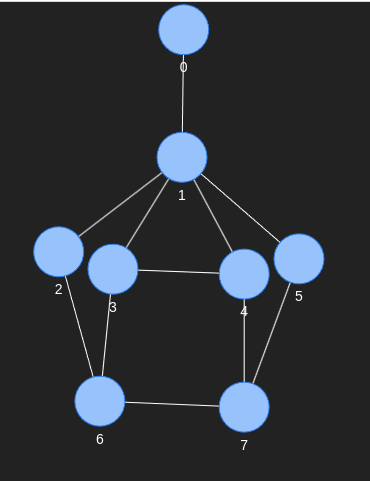
\includegraphics[width=0.4\textwidth]{pictures/at-free-graph-pyvis.png} 
	\caption{To γράφημα εισόδου του Αλγορίθμου σχεδιασμένο από την βιβλιοθήκη PyVis}
	\label{fig:at-free-graph-pyvis}
\end{figure}

\lstinputlisting[
language=text, % or specify another language that suits your needs
breaklines=true,
basicstyle=\footnotesize\ttfamily,
columns=fullflexible,
breakatwhitespace=false,
captionpos=t,
caption={Η εκτέλεση του Αλγορίθμου}
]{Content/CodeDirectory/ind-output.txt}

\begin{figure}[H]
	\centering
	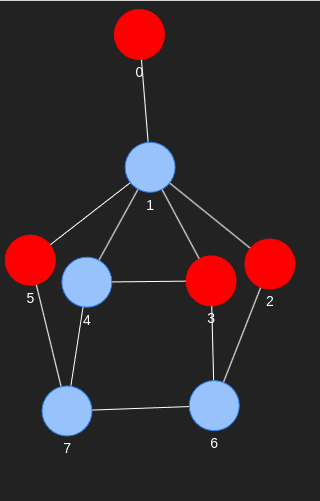
\includegraphics[width=0.4\textwidth]{pictures/at-free-graph-ind-output-pyvis.png} 
	\caption{To γράφημα εξόδου του Αλγορίθμου σχεδιασμένο από την βιβλιοθήκη PyVis}
	\label{fig:at-free-graph-ind-output-pyvis}
\end{figure}


\section{Υπολογισμός Μέγιστου Ανεξάρτητου Συνόλου}
\label{sec:Impl-Independent-set}


Σε αυτό το κεφάλαιο, παρουσιάζουμε συνοπτικά τις κλάσεις που αποτελούν το αλγοριθμικό τμήμα για τον υπολογισμό του μέγιστου ανεξάρτητου συνόλου. Προχωρούμε στην παρουσίαση αυτών των κλάσεων με τη σειρά που χρησιμοποιούνται στο πλαίσιο του συνολικού αλγοριθμικού σχεδιασμού. Επισημαίνουμε ότι αγνοούμε τις κλάσεις που υλοποιούν αλγορίθμους από άλλες εργασίες, όπως ο υπολογισμός ενός ελάχιστου κυρίαρχου μονοπατιού \cite{corneil-olariu-stewart-asteroidal-triple-free-graphs}.



\subsection{H Kλάση PolynomialTimeAlgorithm}


%---------------FILE---------------------------------

\lstinputlisting[
language=Python,
breaklines=true,
basicstyle=\footnotesize\ttfamily,
columns=fullflexible,
breakatwhitespace=false,
captionpos=t,
caption={polynomial\_time\_algorithm.py}
]{Content/CodeDirectory/polynomial_time_algorithm_domination_set.py}
%---------------FILE END---------------------------------

Εξηγούμε αναλυτικά τις συναρτήσεις της κλάσης:

\begin{enumerate}
	\item Κατασκευαστής (\_\_init\_\_): Δέχεται ένα αντικείμενο Graph και ένα ακέραιο weight, που υποδηλώνει το βάρος w αλγορίθμου mcdsw και αρχικοποιεί τα αντίστοιχα χαρακτηριστικά της κλάσης.
	\item Η συνάρτηση \myTTT{mcdsw}: Υλοποιεί τον αλγόριθμο $mcds_{w}$ \ref{alg:domi-set}.
	\item H συνάρτηση \myTTT{initialize\_queue}: Βοηθητική κλάση που αρχικοποιεί την ουρά $A_1$.
	\item H συνάρτηση \myTTT{generate\_subsets}:  H συνάρτηση δημιουργήσει όλα τα υποσύνολα της κλειστής γειτονιάς ενός κόμβου σε μήκη από 1 έως το βάρος (weight) του έχουμε επιλέξει.
\end{enumerate}

\subsection{H Kλάση Graph}

%---------------FILE---------------------------------
\lstinputlisting[
language=Python,
breaklines=true,
basicstyle=\footnotesize\ttfamily,
columns=fullflexible,
breakatwhitespace=false,
captionpos=t,
caption={graph.py}
]{Content/CodeDirectory/graph_domination_set.py}
%---------------FILE END---------------------------------

Εξηγούμε αναλυτικά τις συναρτήσεις της κλάσης:

\begin{enumerate}
	
	\item Μέθοδος \texttt{bfs\_levels}: Υλοποιεί τον αλγόριθμο BFS (Breadth-First Search) για τον υπολογισμό των επιπέδων του γράφου από μια δεδομένη κορυφή.
	
	\item Μέθοδος \texttt{closed\_neighborhood}: Επιστρέφει την κλειστή γειτονιά μιας κορυφής, δηλαδή την κορυφή και όλες τις γειτονικές της κορυφές.
	
	\item Μέθοδος \texttt{closed\_neighborhood\_of\_set}: Υπολογίζει την κλειστή γειτονιά ενός συνόλου κορυφών.
	
	\item Μέθοδος \texttt{show}: Χρησιμοποιεί το πακέτο \texttt{pyvis} για να εμφανίσει το γράφημα σε μορφή διαδραστικού δικτύου.
	
\end{enumerate}

\subsection{Παραδείγματα Εκτέλεσης του Προγράμματος}

Ως παράδειγμα δείχνουμε πως εκτελούμε τον αλγόριθμο υπολογισμού του ελάχιστου κυρίαρχου συνόλου στο ίδιο γράφημα με την Ενότητα \ref{sec:Domination_Set_Alg}. 

\begin{figure}[H]
	\centering
	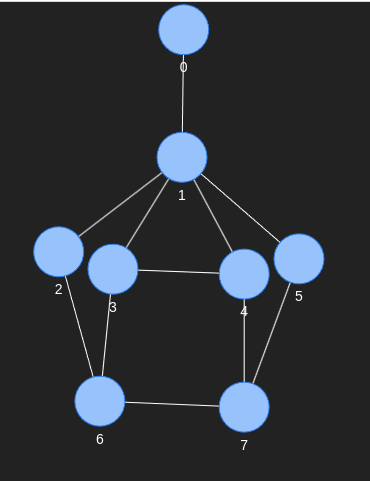
\includegraphics[width=0.4\textwidth]{pictures/at-free-graph-pyvis.png} 
	\caption{To γράφημα εισόδου του Αλγορίθμου σχεδιασμένο από την βιβλιοθήκη PyVis}
\end{figure}

\lstinputlisting[
language=text, % or specify another language that suits your needs
breaklines=true,
basicstyle=\footnotesize\ttfamily,
columns=fullflexible,
breakatwhitespace=false,
captionpos=t,
caption={Η εκτέλεση του Αλγορίθμου}
]{Content/CodeDirectory/domi-output.txt}


\begin{figure}[H]
	\centering
	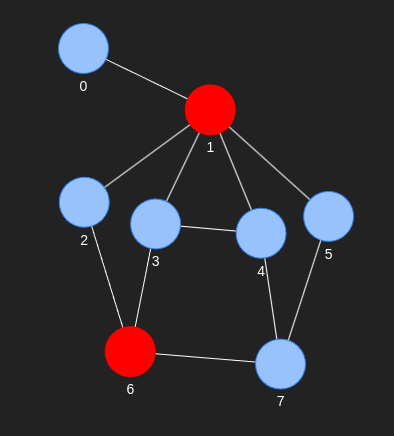
\includegraphics[width=0.4\textwidth]{pictures/at-free-graph-domi-output-pyvis.png} 
	\caption{To γράφημα εξόδου του Αλγορίθμου σχεδιασμένο από την βιβλιοθήκη PyVis}
\end{figure}

\section{Το Πρόβλημα του 3-Χρωματισμού}

Στο παρόν κεφάλαιο, παρουσιάζουμε ενδεικτικές κλάσεις που αποτελούν το αλγοριθμικό τμήμα για την επίλυση του προβλήματος 3-χρωματισμού. Προχωρούμε στην παρουσίαση αυτών των κλάσεων με τη σειρά που καλούνται στο πλαίσιο του συνολικού αλγοριθμικού σχεδιασμού. Σημειώνουμε πως παραλείπουμε τις κλάσεις που υλοποιούν αλγορίθμους από άλλες εργασίες, όπως ο Αλγόριθμος "Biconnectivity" του Robert Tarjan \cite{tarjan-depth-first-search}.

\subsection{H Kλάση PolynomialTimeAlgorithm}


%---------------FILE---------------------------------

\lstinputlisting[
language=Python,
breaklines=true,
basicstyle=\footnotesize\ttfamily,
columns=fullflexible,
breakatwhitespace=false,
captionpos=t,
caption={polynomial\_time\_algorithm.py}
]{Content/CodeDirectory/polynomial_time_algorithm_3_colouring.py}
%---------------FILE END---------------------------------

Εξηγούμε τις συναρτήσεις της κλάσης:

\begin{enumerate}
	\item Κατασκευαστής (\_\_init\_\_): Δέχεται ένα αντικείμενο Graph και αρχικοποιεί μερικές μεταβλητές που θα χρειαστούν για την σωστή λειτουργία του αλγορίθμου.
	
	\item H συνάρτηση \myTTT{three\_colouring}: Είναι η κύρια συνάρτηση που εκτελεί τα βήματα του αλγορίθμου για την επίλυση του προβλήματος 3-Χρωματισμού.
	
	\item Η συνάρτηση \myTTT{line\_1\_check}: Υλοποιεί τον έλεγχο της πρώτης γραμμής του αλγορίθμου.: Ελέγχει αν υπάρχει κύκλος μεγέθους 4 ($K_4$) στο $G$.
	
	\item H συνάρτηση \myTTT{line\_5\_check}: Ελέγχει αν υπάρχει διαμάντι στον γράφημα.    
	
	\item H συνάρτηση \myTTT{line\_9\_check}:  Ελέγχει αν υπάρχει ελάχιστο σταθερό διαχωριστής στο γράφημα.
	
	\item H συνάρτηση \myTTT{perform\_contraction}:  Βοηθητική συνάρτηση που εκτελεί σύμπτυξη δύο κορυφών.
\end{enumerate}

\subsection{H Kλάση Graph}


%---------------FILE---------------------------------

\lstinputlisting[
language=Python,
breaklines=true,
basicstyle=\footnotesize\ttfamily,
columns=fullflexible,
breakatwhitespace=false,
captionpos=t,
caption={graph.py}
]{Content/CodeDirectory/graph_3_colouring.py}
%---------------FILE END---------------------------------

Εξηγούμε τις συναρτήσεις της κλάσης:

\begin{enumerate}
	\item \texttt{is\_triangle}: Ελέγχει εάν το γράφημα είναι τρίγωνο, δηλαδή αν έχει 3 κορυφές ή 3 ακμές.
	
	\item \texttt{find\_K4}: Ελέγχει εάν το γράφημα περιέχει ένα $K_4$.
	
	\item \texttt{find\_triangle\_in\_neighborhood}: Ελέγχει εάν η γειτονιά μιας συγκεκριμένης κορυφής περιέχει τρίγωνο. Αυτή η συνάρτηση καλείται για τον έλεγχο της γραμμής 1 του αλγορίθμου μετά από αναδρομή. 
	
	\item \texttt{find\_diamond}: Η συνάρτηση ψάχνει να βρει άμα υπάρχει διαμάντι στο γράφημα, βρίσκοντας δύο κορυφές που έχουν τουλάχιστον δύο κοινούς γείτονες.
	
	\item \texttt{contract}: Συμπτύσσει ένα σύνολο κορυφών σε μια μοναδική κορυφή.
	
	\item \texttt{delete\_vertices}: Διαγράφει ένα σύνολο κορυφών από το γρφημα.
	
	\item \texttt{edge\_exists}: Ελέγχει εάν μια ακμή υπάρχει στο γράφημα.
	
	\item \texttt{copy}: Δημιουργεί αντίγραφο του γράφου.
	
	\item \texttt{show}: Εμφανίζει το γράφημα χρησιμοποιώντας τη βιβλιοθήκη pyvis σε μορφή διαδραστικού δικτύου.
\end{enumerate}


\subsection{H Kλάση Block}

Η κλάση Block αναπαριστά τα μπλοκς του αλγορίθμου. Περιλαμβάνει μεθόδους για την εύρεση ελάχιστων σταθερών διαχωριστών και τον έλεγχο της συνδεσιμότητας

%---------------FILE---------------------------------

\lstinputlisting[
language=Python,
breaklines=true,
basicstyle=\footnotesize\ttfamily,
columns=fullflexible,
breakatwhitespace=false,
captionpos=t,
caption={block.py}
]{Content/CodeDirectory/block.py}
%---------------FILE END---------------------------------

Εξηγούμε τις συναρτήσεις της κλάσης:

\begin{enumerate}
	\item \texttt{find\_minimal\_stable\_separator}: Αναζητά τον ελάχιστο σταθερό διαχωριστικό σε έναν κόμβο $x$.
	
	\item \texttt{find\_stable\_cutset}: Ελέγχει εάν μια συγκεκριμένη γειτονιά του κόμβου $x$ είναι ένα σταθερό διαχωριστικό.
	
	\item \texttt{reduce\_cutset\_to\_minimal\_stable\_separator}: Μειώνει ένα διαχωριστικό σύνολο σε ένα ελάχιστο σταθερό διαχωριστικό.
	
	\item \texttt{delete\_vertices}: Διαγράφει ένα σύνολο κορυφών από το μπλοκ.
	
	\item \texttt{is\_connected}: Ελέγχει εάν το μπλοκ είναι συνδεδεμένο.
	
	\item \texttt{dfs}: Υλοποιεί τον αλγόριθμο του "Depth-first search" για να ελέγξει τη συνδεσιμότητα του μπλοκ.
	
	\item \texttt{copy}: Δημιουργεί αντίγραφο του μπλοκ.
\end{enumerate}

\subsection{H Kλάση ThreeColouring}

Η κλάση ThreeColouring χρωματίζει με τρία χρώματα το συμπτυγμένο γράφημα που προκύπτει στην γραμμή 13 του αλγορίθμου \ref{alg:coloring}.


%---------------FILE---------------------------------

\lstinputlisting[
language=Python,
breaklines=true,
basicstyle=\footnotesize\ttfamily,
columns=fullflexible,
breakatwhitespace=false,
captionpos=t,
caption={three\_colouring.py}
]{Content/CodeDirectory/colouring.py}
%---------------FILE END---------------------------------

Εξηγούμε τις συναρτήσεις της κλάσης:


\begin{enumerate}
	\item \texttt{construct\_three\_colouring}: Είναι η βασική συνάρτηση χρωματισμού του γραφήματος. Αρχικά ελέγχει πόσα μπλοκς υπάρχουν στο γράφημα. Αν είναι περισσότερα από ένα υπολογίζει ένα δέντρο για με τα μπλοκς χρησιμοποιώντας τα cutpoints του γραφήματος.
	
	\item \texttt{colour\_triangle}: Χρωματίζει ένα τρίγωνο με τρία διαφορετικά χρώματα.
	
	\item \texttt{colour\_triangular\_strip}: Χρωματίζει μια τριγωνική λωρίδα με τρία χρώματα.
	
	\item \texttt{find\_init\_triangle\_in\_strip}: Εντοπίζει το αρχικό τρίγωνο σε μια τριγωνική λωρίδα.
	
	\item \texttt{find\_triangle\_in\_strip}: Βρίσκει ένα τρίγωνο σε μια τριγωνική λωρίδα, ξεκινώντας από μια δεδομένη κορυφή.
	
	\item \texttt{colour\_triangle\_of\_triangular\_strip}: Χρωματίζει ένα τρίγωνο μιας τριγωνικής λωρίδας.
	
	\item \texttt{colour\_prism}: Χρωματίζει ένα πρίσμα, δηλαδή μια τριγωνικό λωρίδα τάξης 2.
	
	\item \texttt{find\_triangles\_in\_prism}: Εντοπίζει τα δύο τρίγωνα σε ένα πρίσμα.
	
	\item \texttt{colour\_remaining\_vertices}: Χρωματίζει τις κορυφές του γραφήματος που δεν ανήκουν σε κάποιο μπλοκ, χρησιμοποιώντας τρία χρώματα και αποφεύγοντας τις συγκρούσεις χρωμάτων.
	
	\item \texttt{colour\_initial\_graph}: Χρωματίζει το αρχικό γράφημα από το συμπαγές. 
		
\end{enumerate}

\subsection{H Kλάση BlockCutpointTree}


%---------------FILE---------------------------------

\lstinputlisting[
language=Python,
breaklines=true,
basicstyle=\footnotesize\ttfamily,
columns=fullflexible,
breakatwhitespace=false,
captionpos=t,
caption={block\_cutpoint\_tree.py}
]{Content/CodeDirectory/tree.py}
%---------------FILE END---------------------------------

Εξηγούμε τις συναρτήσεις της κλάσης:

\begin{enumerate}
	\item \texttt{\_\_init\_\_}: Ο κατασκευαστής της κλάσης που αρχικοποιεί τις μεταβλητές blocks, cutpoints, root, tree και visited.
	
	\item \texttt{create\_tree}: Δημιουργεί το δέντρο απόφασης (Block-Cutpoint Tree) βασισμένο στα μπλοκ και τα cutpoints. Δημιουργεί έναν κόμβο για κάθε μπλοκ και συνδέει με ακμές τους κόμβους που αντιστοιχούν σε μπλοκ που περιέχουν το ίδιο cutpoint.
	
	\item \texttt{get\_next\_block}: Επιστρέφει τον επόμενο μη επισκεπτημένο κόμβο του δέντρου Block-Cutpoint Tree. Χρησιμοποιείται για τον εντοπισμό επόμενου μπλοκ που πρέπει να εξεταστεί.
	
	\item \texttt{show}: Εμφανίζει γραφικά το δέντρο Block-Cutpoint Tree.
\end{enumerate}


\subsection{Παραδείγματα Εκτέλεσης του Προγράμματος}

Ως παράδειγμα δείχνουμε πως εκτελούμε τον αλγόριθμο 3-χρωματισμού στο ίδιο γράφημα με την Ενότητα \ref{sec:3-Coloring_Alg}. 

%---------------FILE---------------------------------
\lstinputlisting[
language=json,
breaklines=true,
basicstyle=\footnotesize\ttfamily,
columns=fullflexible,
breakatwhitespace=false,
captionpos=t,
caption={Το γράφημα σε μορφή JSOn}
]{Content/CodeDirectory/input-graph-colouring.json}
%---------------FILE END---------------------------------

\begin{figure}[H]
	\centering
	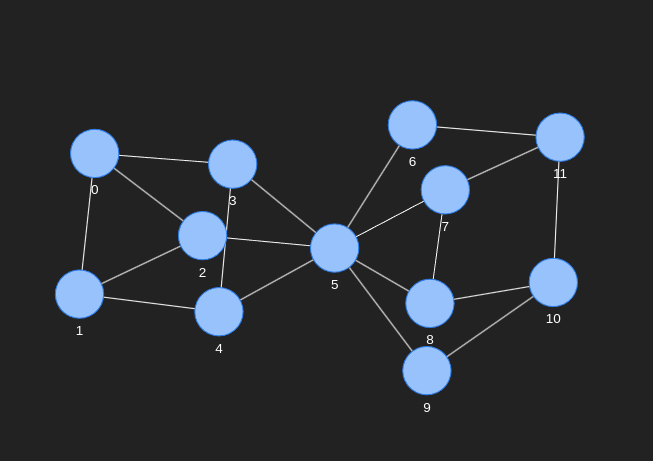
\includegraphics[width=0.7\textwidth]{pictures/coloring-1.png} 
	\caption{To γράφημα εισόδου του Αλγορίθμου σχεδιασμένο από την βιβλιοθήκη PyVis}
	\label{fig:at-free-graph-pyvis-3-colouring}
\end{figure}

Παρακάτω δείχνουμε όλα τα στιγμιότυπα του γραφήματος κατά την διάρκεια εκτέλεσης του αλγορίθμου.

\begin{figure}[H]
	\centering
	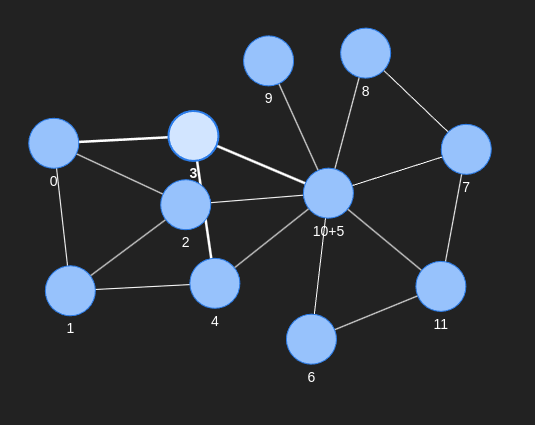
\includegraphics[width=0.7\textwidth]{pictures/coloring-2.png} 
	\caption{To γράφημα μετά την σύμπτυξη των κορυφών 10,5}
	\label{fig:at-free-graph-pyvis-3-colouring-2}
\end{figure}

\begin{figure}[H]
	\centering
	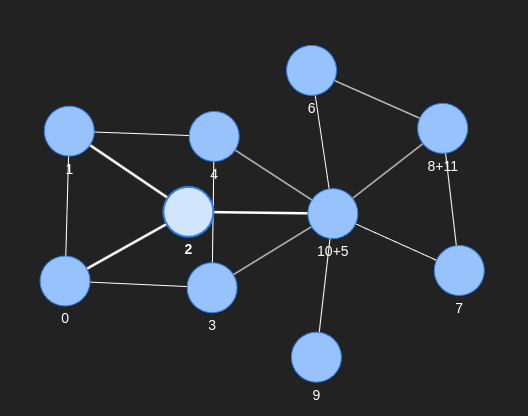
\includegraphics[width=0.7\textwidth]{pictures/coloring-3.png} 
	\caption{To γράφημα μετά την σύμπτυξη των κορυφών 8,11}
	\label{fig:at-free-graph-pyvis-3-colouring-3}
\end{figure}

\begin{figure}[H]
	\centering
	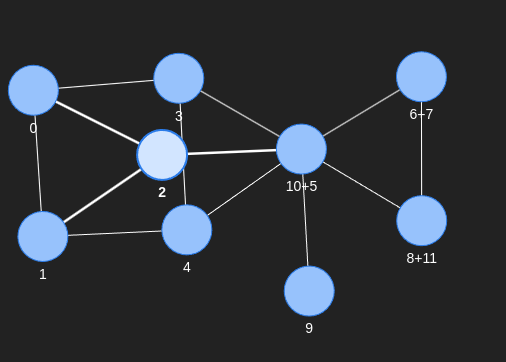
\includegraphics[width=0.7\textwidth]{pictures/coloring-4.png} 
	\caption{To γράφημα μετά την σύμπτυξη των κορυφών 7,6}
	\label{fig:at-free-graph-pyvis-3-colouring-4}
\end{figure}

\begin{figure}[H]
	\centering
	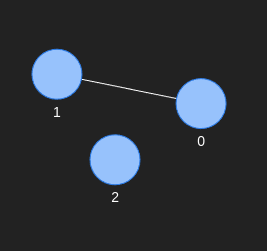
\includegraphics[width=0.3\textwidth]{pictures/coloring-block-cutpoint.png} 
	\caption{ Block Cutpoint Tree \{ 0: \{8+11,6+7,10+5\}, 1: \{1,10+5,2,3,4,0\}, 2: \{9\}\}}
	\label{fig:at-free-graph-pyvis-3-colouring-block-cutpoint}
\end{figure}


\begin{figure}[H]
	\centering
	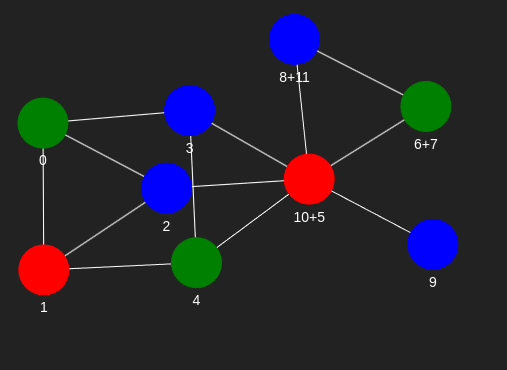
\includegraphics[width=0.7\textwidth]{pictures/coloring-before-expansion.png} 
	\caption{To "συμπτυγμένο" γράφημα μετά τον 3-χρωματισμό}
	\label{fig:at-free-graph-pyvis-3-colouring-before-expansion}
\end{figure}

\begin{figure}[H]
	\centering
	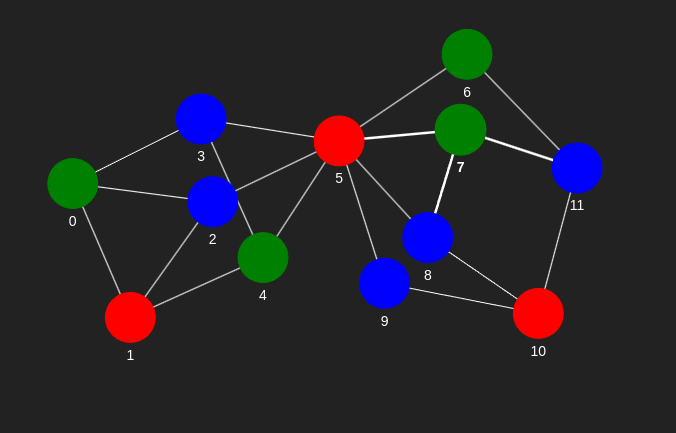
\includegraphics[width=0.7\textwidth]{pictures/coloring-final.png} 
	\caption{To γράφημα μετά το τέλος του αλγορίθμου}
	\label{fig:at-free-graph-pyvis-3-colouring-final}
\end{figure}
